\documentclass[tikz, border=5pt]{standalone}
\usetikzlibrary{shapes.geometric, arrows.meta, positioning, fit, backgrounds, shadows}
\usepackage{amsmath}

\begin{document}

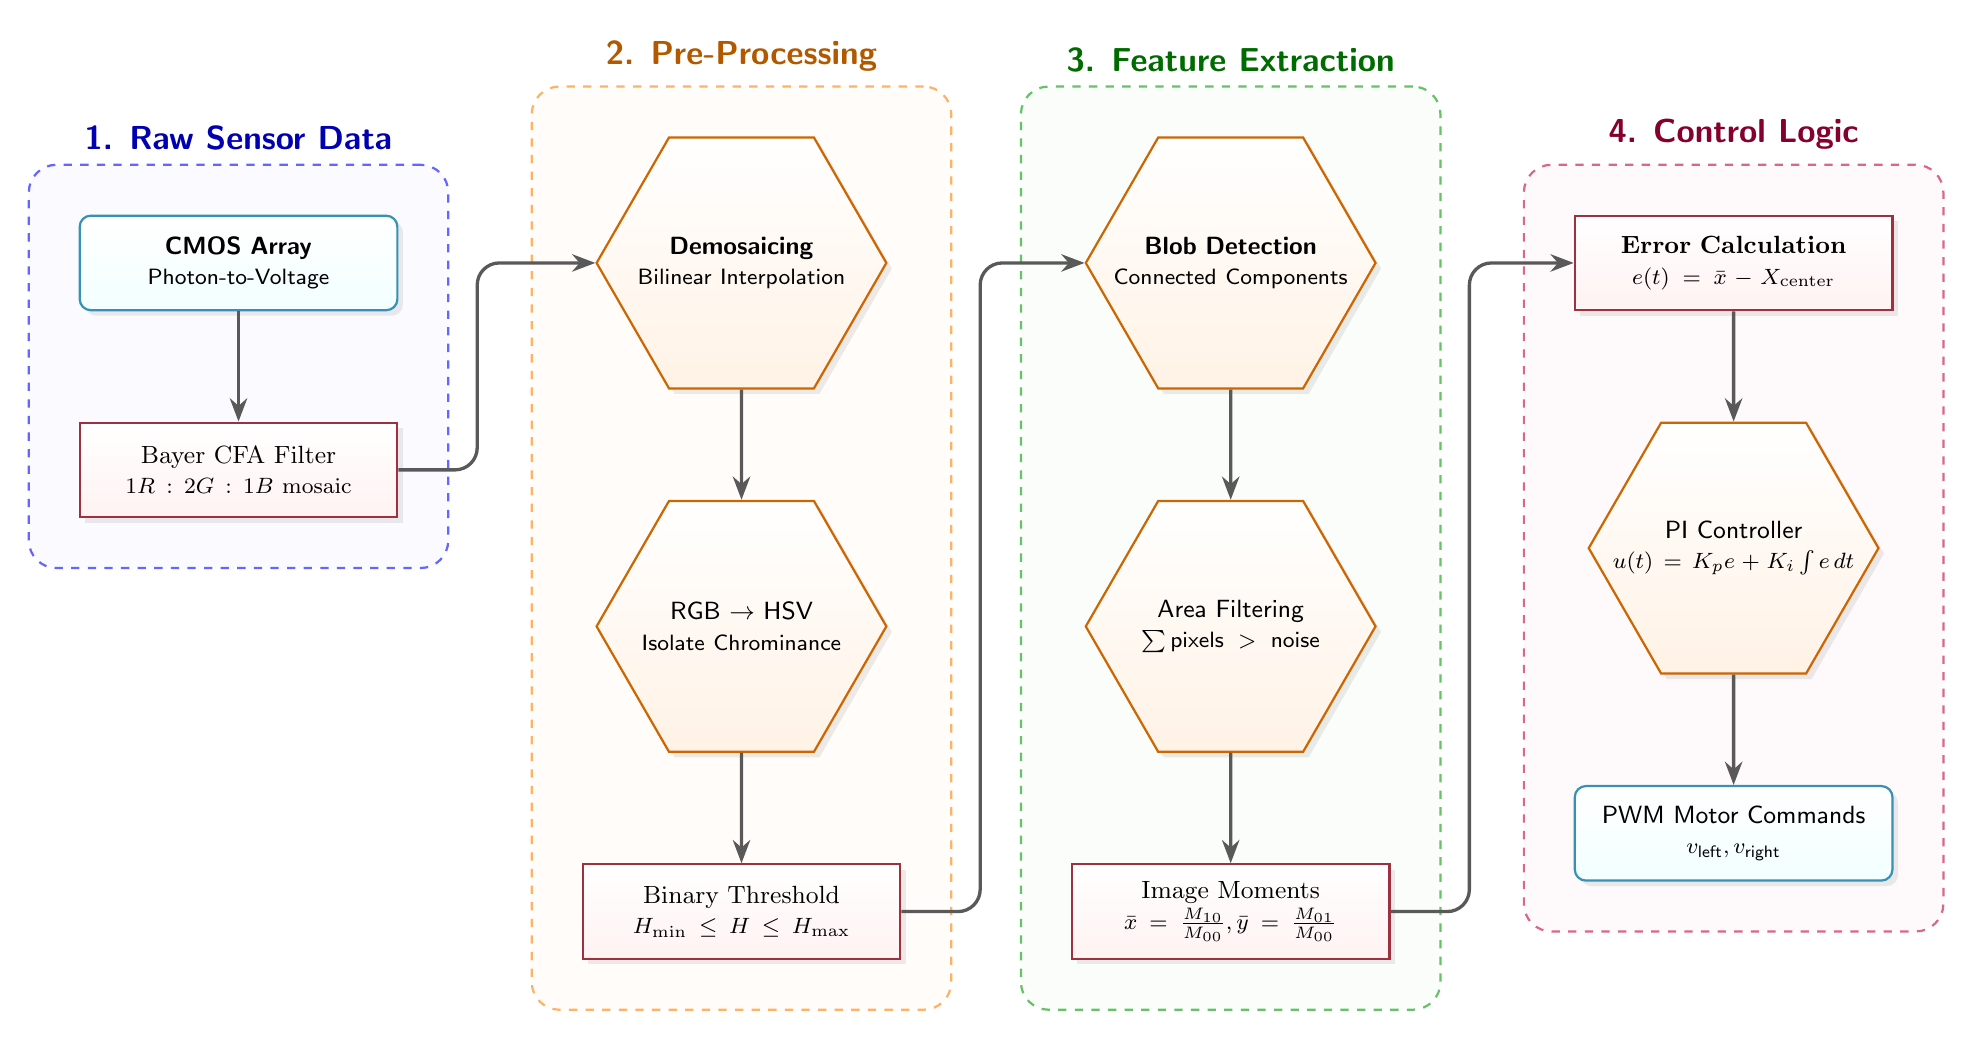
\begin{tikzpicture}[
    % Increased horizontal distance to give the inter-stage arrows room to breathe
    node distance=1.4cm and 2.5cm, 
    >=Stealth,
    font=\sffamily\small,
    % --- Style Definitions ---
    stagebox/.style={
        rectangle, rounded corners=10pt, 
        draw=#1!60, fill=#1!2, 
        dashed, thick, inner sep=18pt
    },
    header/.style={
        font=\sffamily\bfseries\large, 
        text=#1!70!black, 
        inner sep=5pt
    },
    common/.style={
        text width=3.8cm, 
        align=center, 
        minimum height=1.2cm,
        drop shadow={opacity=0.15, shadow xshift=2pt, shadow yshift=-2pt}
    },
    datanode/.style={
        common, rectangle, rounded corners=4pt,
        draw=cyan!70!black, fill=white, 
        top color=white, bottom color=cyan!5, thick
    },
    processnode/.style={
        common, regular polygon, regular polygon sides=6,
        draw=orange!80!black, fill=white, 
        top color=white, bottom color=orange!10, thick,
        inner sep=-22pt 
    },
    mathnode/.style={
        common, rectangle, 
        draw=rose!70!black, fill=white, 
        top color=white, bottom color=red!5, thick,
        font=\small 
    },
    arrow/.style={
        ->, line width=1.2pt, color=gray!70!black, 
        rounded corners=8pt
    }
]

% Define a custom color
\definecolor{rose}{RGB}{225, 70, 90}

% ================= Stage 1: Raw Sensor =================
\node[datanode] (cmos) {\textbf{CMOS Array}\\ \footnotesize Photon-to-Voltage};
\node[mathnode, below=of cmos] (bayer) {Bayer CFA Filter\\ \footnotesize $1R:2G:1B$ mosaic};

% ================= Stage 2: Pre-Processing =================
\node[processnode, right=of cmos] (demosaic) {\textbf{Demosaicing}\\ \footnotesize Bilinear Interpolation};
\node[processnode, below=of demosaic] (hsv) {RGB $\to$ HSV\\ \footnotesize Isolate Chrominance};
\node[mathnode, below=of hsv] (thresh) {Binary Threshold\\ \footnotesize $H_{\min} \le H \le H_{\max}$};

% ================= Stage 3: Feature Extraction =================
\node[processnode, right=of demosaic] (ccl) {\textbf{Blob Detection}\\ \footnotesize Connected Components};
\node[processnode, below=of ccl] (filter) {Area Filtering\\ \footnotesize $\sum \text{pixels} > \text{noise}$};
\node[mathnode, below=of filter] (moments) {Image Moments\\ \footnotesize $\bar{x} = \frac{M_{10}}{M_{00}}, \bar{y} = \frac{M_{01}}{M_{00}}$};

% ================= Stage 4: Control Logic =================
\node[mathnode, right=of ccl] (error) {\textbf{Error Calculation}\\ \footnotesize $e(t) = \bar{x} - X_{\text{center}}$};
\node[processnode, below=of error] (pi) {PI Controller\\ \footnotesize $u(t) = K_p e + K_i \int e \, dt$};
\node[datanode, below=of pi] (motors) {PWM Motor Commands\\ \footnotesize $v_{\text{left}}, v_{\text{right}}$};

% ================= Background & Headers =================
\begin{scope}[on background layer]
    \node[stagebox=blue, fit=(cmos) (bayer)] (group1) {};
    \node[header=blue, above=0pt of group1] {1. Raw Sensor Data};

    \node[stagebox=orange, fit=(demosaic) (thresh)] (group2) {};
    \node[header=orange, above=0pt of group2] {2. Pre-Processing};

    \node[stagebox=green!60!black, fit=(ccl) (moments)] (group3) {};
    \node[header=green!60!black, above=0pt of group3] {3. Feature Extraction};

    \node[stagebox=purple, fit=(error) (motors)] (group4) {};
    \node[header=purple, above=0pt of group4] {4. Control Logic};
\end{scope}

% ================= Connection Logic =================
% Intra-stage (Straight down)
\draw[arrow] (cmos) -- (bayer);
\draw[arrow] (demosaic) -- (hsv); \draw[arrow] (hsv) -- (thresh);
\draw[arrow] (ccl) -- (filter); \draw[arrow] (filter) -- (moments);
\draw[arrow] (error) -- (pi); \draw[arrow] (pi) -- (motors);

% Inter-stage (Clean East-to-West snake routing)
% The line goes right by 1cm, then up to the correct Y-level, then right into the next node.
\draw[arrow] (bayer.east) -- ++(1,0) |- (demosaic.west);
\draw[arrow] (thresh.east) -- ++(1,0) |- (ccl.west);
\draw[arrow] (moments.east) -- ++(1,0) |- (error.west);

\end{tikzpicture}
\end{document}